\documentclass[main.tex]{subfiles}
\begin{document}\newpage
\setdoublesep{0.35700 em}  % 'Bond Spacing'
\setatomsep{1.78500 em}    % 'Fixed Length'
\setbondoffset{0.18265 em} % 'Margin Width'
\newcommand{\bondwidth}{0.06642 em} % 'Line Width'
\setbondstyle{line width = \bondwidth}
\newgeometry{left=0.8in,right=0.8in, top=2.5cm,bottom=2cm}
\fancyhfoffset[E,O]{0pt}
\setlength{\columnsep}{30pt}
\begin{conclusion}
\end{conclusion}
%\setstretch{0.3}
\begin{multicols*}{2}\setcounter{numA}{1}



{\raggedright\textsc{\textbf{Chemical Equilibrium }}\par}
%%%%%PROBLEM
\begin{question}[ID=\the\value{numA}]\SetQuestionProperties{section-title=\nameref{sec:units}}
Write down the forward and reverse reactions for the following reactions in equilibrium:\begin{enumerate}[label=(\alph*)]	
\item   \ce{CH4_{(g)} + O2_{(g)} <=> CO2_{(g)} + H2O_{(g)}}
\item \ce{2Mg_{(s)} + O2_{(g)} <=> 2MgO_{(s)}}
 \end{enumerate}
\end{question}
\begin{solution}
\begin{inparaenum}[(a)]
\item   \ce{CH4_{(g)} + O2_{(g)} -> CO2_{(g)} + H2O_{(g)}}; \ce{CH4_{(g)} + O2_{(g)} <- CO2_{(g)} + H2O_{(g)}}
\item \ce{2Mg_{(s)} + O2_{(g)} -> 2MgO_{(s)}};\ce{2Mg_{(s)} + O2_{(g)} <- 2MgO_{(s)}}
 \end{inparaenum}
\hspace{0.1cm}\end{solution}\stepcounter{numA}%%%%%%%%%%%%



{\raggedright\textsc{\textbf{Equilibrium constants }}\par}



%%%%%PROBLEM
\begin{question}[ID=\the\value{numA}]\SetQuestionProperties{section-title=\nameref{sec:units}}
For the reactions below and given the value of the equilibrium constant indicate whether the equilibrium mixture will have:
\begin{inparaenum}[(a)]	
\item More reactants than products
\item More  products than reactants
\item Same amount of  products and reactants
 \end{inparaenum}
 \begin{enumerate}[label=(\alph*)]	
\item   \ce{CO2_{(g)} + H2O_{(g)} <=>  CH4_{(g)} + O2_{(g)}  }\hfill $K_{c}=0.001$ %More reactants
\item \ce{N2_{(g)} + O2_{(g)} <=> 2NO_{(g)}}\hfill$K_{c}=2\cdot 10^{25}$	%More products
\item \ce{2NO_{(g)} + O2_{(g)} <=> 2NO2_{(g)}}\hfill $K_{c}=6.4\cdot 10^{9}$	%More products

 \end{enumerate}
\end{question}
\begin{solution}
\begin{inparaenum}[(a)]
\item    More reactants
\item  More products
\item  More products
 \end{inparaenum}
\hspace{0.1cm}\end{solution}\stepcounter{numA}%%%%%%%%%%%%


%%%%%PROBLEM
\begin{question}[ID=\the\value{numA}]\SetQuestionProperties{section-title=\nameref{sec:units}}
For the reactions below and given the value of the equilibrium constant indicate whether the equilibrium mixture will have:
\begin{inparaenum}[(a)]	
\item More reactants than products
\item More  products than reactants
\item Same amount of  products and reactants
 \end{inparaenum}
 \begin{enumerate}[label=(\alph*)]	
\item \ce{N2_{(g)} + 3H2_{(g)} <=> 2NH3_{(g)}}\hfill$K_{c}=1$	%same amount
\item	\ce{2NO_{(g)} + Cl2_{(g)} <=> 2NOCl_{(g)}}\hfill $K_{c}=6.5\cdot 10^{4}$ % More products
 \end{enumerate}
\end{question}
\begin{solution}
\begin{inparaenum}[(a)]
\item  same amount
\item	  More products
 \end{inparaenum}
\hspace{0.1cm}\end{solution}\stepcounter{numA}%%%%%%%%%%%%


%%%%%PROBLEM
\begin{question}[ID=\the\value{numA}]\SetQuestionProperties{section-title=\nameref{sec:units}}
Write down the expression of $K_{c}$ for the following reaction:
 \begin{enumerate}[label=(\alph*)]	
\item  \ce{2SO2_{(g)} + O2_{(g)} <=> 2SO3_{(g)}} % $K_{c}=\frac{   \big[ \ce{SO3} \big]^2    } { \big[\ce{SO2} \big]^2 \cdot \big[\ce{O2} \big]\  } $
\item  \ce{CO_{(g)} + 2H2_{(g)} <=> CH3OH_{(g)}} % $K_{c}=\frac{  \big[\ce{CH3OH} \big]  } { \big[\ce{H2} \big]^2 \cdot \big[\ce{CO} \big]\  } $
\item  \ce{C2H6_{(g)} + Cl2_{(g)} <=> C2H2Cl_{(s)} + HCl_{(g)}} %$K_{c}=\frac{   \big[ \ce{HCl} \big]    } { \big[\ce{C2H6} \big] \cdot \big[\ce{Cl2} \big]\  } $
 \end{enumerate}
\end{question}
\begin{solution}
\begin{inparaenum}[(a)]
\item    $K_{c}=\frac{   \big[ \ce{SO3} \big]^2    } { \big[\ce{SO2} \big]^2 \cdot \big[\ce{O2} \big]\  } $ ; $K_{p}=\frac{   p_{\ce{SO3}}^2    } { p_{\ce{SO2}}^2 \cdot p_{\ce{O2}}  } $
\item    $K_{c}=\frac{  \big[\ce{CH3OH} \big]  } { \big[\ce{H2} \big]^2 \cdot \big[\ce{CO} \big]\  } $;$K_{p}=\frac{  p_{\ce{CH3OH}}   } { p_{\ce{H2}}^2 \cdot p_{\ce{CO}}  } $
\item  $K_{c}=\frac{   \big[ \ce{HCl} \big]    } { \big[\ce{C2H6} \big] \cdot \big[\ce{Cl2} \big]\  } $ ; $K_{p}=\frac{   p_{ \ce{HCl}}    } { p_{\ce{C2H6}}  \cdot p_{\ce{Cl2}}   } $
 \end{inparaenum}
\hspace{0.1cm}\end{solution}\stepcounter{numA}%%%%%%%%%%%%




%%%%%PROBLEM
\begin{question}[ID=\the\value{numA}]\SetQuestionProperties{section-title=\nameref{sec:units}}
Write down the expression of $K_c$ for the following reaction:
 \begin{enumerate}[label=(\alph*)]	
\item \ce{BaCO3_{(s)} <=> Ba^{2+}_{(aq)} + CO3^{2-}_{(aq)}} % $\big[\ce{Ba^{2+}}\big] \cdot \big[\ce{CO3^{2-}} \big]\  $
\item \ce{2H2_{(g)} + O2_{(g)} <=> 2H2O_{(l)}} %$\frac{  1  } { \big[\ce{H2} \big]^2 \cdot \big[\ce{O2} \big]\  } $
 \end{enumerate}
\end{question}
\begin{solution}
\begin{inparaenum}[(a)]
\item   $\big[\ce{Ba^{2+}}\big] \cdot \big[\ce{CO3^{2-}} \big]\  $
\item  $\frac{  1  } { \big[\ce{H2} \big]^2 \cdot \big[\ce{O2} \big]\  } $
 \end{inparaenum}
\hspace{0.1cm}\end{solution}\stepcounter{numA}%%%%%%%%%%%%



%%%%%PROBLEM
\begin{question}[ID=\the\value{numA}]\SetQuestionProperties{section-title=\nameref{sec:units}}
Indicate which of the following diagrams represent better the system at equilibrium:
 \begin{center}\includegraphics[width=0.4\textwidth]{./chapter18/figure10}\end{center}
 \begin{enumerate}[label=(\alph*)]	
\item	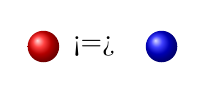
\begin{tikzpicture} \shade [ball color=red] (0:0.5) circle (0.2cm) node [shift={(2em,0)}] { \ce{<=> } } ; \shade [ball color=blue] (0:2.0) circle (0.2cm);\end{tikzpicture} \hfill $K_{c}=10$  % Left
\item	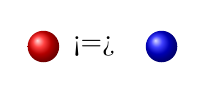
\begin{tikzpicture} \shade [ball color=red] (0:0.5) circle (0.2cm) node [shift={(2em,0)}] { \ce{<=> } } ; \shade [ball color=blue] (0:2.0) circle (0.2cm);\end{tikzpicture} \hfill $K_{c}=0.1$  % Right
\item	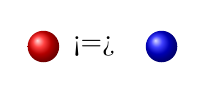
\begin{tikzpicture} \shade [ball color=red] (0:0.5) circle (0.2cm) node [shift={(2em,0)}] { \ce{<=> } } ; \shade [ball color=blue] (0:2.0) circle (0.2cm);\end{tikzpicture} \hfill $K_{c}=1$  % Center
 \end{enumerate}
\end{question}
\begin{solution}
\begin{inparaenum}[(a)]
\item  Left
\item   Right
\item   Center
 \end{inparaenum}
\hspace{0.1cm}\end{solution}\stepcounter{numA}%%%%%%%%%%%%

%%%%%PROBLEM
\begin{question}[ID=\the\value{numA}]\SetQuestionProperties{section-title=\nameref{sec:units}}
Complete the table and calculate $K_c$ and $K_p$ at 300K:
\begin{center}\begin{tabular}[t]{  c c  c       }
\toprule
Reaction	&	$K_c$  	&		$K_p$ \\
\midrule
\ce{2NH3_{(g)}  <=> N2_{(g)}	+ 3H2_{(g)}} &	17	&	 	\\
\ce{2SO3_{(g)}  <=> 2SO2_{(g)} + O2_{(g)}} &	0.243	&	 	\\
\ce{SO2Cl2_{(g)} <=> SO2_{(g)} + Cl2_{(g)}} &		&0.05	 	\\
\ce{Cl2_{(g)}	+ Br2_{(g)}  <=>	 2BrCl2_{(g)} } &		&0.196	 	\\
\bottomrule
\end{tabular}\end{center}
 \end{question}
\begin{solution}
\begin{center}\begin{tabular}[t]{  c c  c       }
\toprule
Reaction	&	$K_c$  	&		$K_p$ \\
\midrule
\ce{2NH3_{(g)}  <=> N2_{(g)}	+ 3H2_{(g)}} &	17	&10288	 	\\
\ce{2SO3_{(g)}  <=> 2SO2_{(g)} + O2_{(g)}} &	0.243	&5.977	 	\\
\ce{SO2Cl2_{(g)} <=> SO2_{(g)} + Cl2_{(g)}} &	$2\times 10^{-3}$	&0.05	 	\\
\ce{Cl2_{(g)}	+ Br2_{(g)}  <=>	 2BrCl2_{(g)} } &0.196		&0.196	 	\\
\bottomrule
\end{tabular}\end{center}
\hspace{0.1cm}\end{solution}\stepcounter{numA}%%%%%%%%%%%%







{\raggedright\textsc{\textbf{Using equilibrium constants }}\par}


%%%%%PROBLEM
\begin{question}[ID=\the\value{numA}]\SetQuestionProperties{section-title=\nameref{sec:units}}
The reaction of carbon monoxode with hydrogen to produce methanol has a equilibrium constant in terms of concentration that at a certain temperature is larger than one
\begin{center}\ce{CO(g) + 2H2(g) <=> CH3OH(g)} \hfill  $K_{c}=14.5$\end{center}
Calculate:
\begin{inparaenum}[(a)]
\item the equilibrium concentration of hydrogen (\ce{H2}) given that the equilibrium concentration of methanol (\ce{CH3OH}) and hydrogen (\ce{H2}) for the reaction is 2M, respectively. %0.034 M
\item the equilibrium concentration of hydrogen (\ce{H2}) given that the equilibrium concentration of methanol (\ce{CH3OH}) and carbon dioxide (\ce{CO}) for the reaction are 3M and 1M, respectively.  %0.46M
 \end{inparaenum}
\end{question}
\begin{solution}
\begin{inparaenum}[(a)]
\item  0.034 M
\item  0.46M
 \end{inparaenum}\hspace{0.1cm}\end{solution}\stepcounter{numA}%%%%%%%%%%%%




%%%%%PROBLEM
\begin{question}[ID=\the\value{numA}]\SetQuestionProperties{section-title=\nameref{sec:units}}
Consider the following reaction:
\begin{center}\ce{2SO2(g) + O2(g) <=> 2SO3(g)}\end{center}
\begin{inparaenum}[(a)]
\item Write down the expression of $K$.
\item Calculate the numerical value of $K$ for the reaction if the concentrations at equilibrium at 1000K are 2M for \ce{SO3}, 0.3M for \ce{O2} and 1M for \ce{SO2}.
\item indicate whether an equilibrium mixture will contain mostly products, mostly reactants or maybe both.
 \end{inparaenum}
\end{question}
\begin{solution}
\begin{inparaenum}[(a)]
\item $\frac{  \big[\ce{SO3} \big]^2  } { \big[\ce{SO2} \big]^2 \cdot \big[\ce{O2} \big]\  } $
\item 3.4
\item mostly products
 \end{inparaenum}
\hspace{0.1cm}\end{solution}\stepcounter{numA}%%%%%%%%%%%%

{\raggedright\textsc{\textbf{Concentration ratio }}\par}

%%%%%PROBLEM
\begin{question}[ID=\the\value{numA}]\SetQuestionProperties{section-title=\nameref{sec:units}}
For the reactions below indicate whether they will evolve towards the right or towards the left in order to reach equilibrium.
\begin{center}\begin{tabular}[t]{  l c  c        }
\toprule
Reaction	&	$K_c$  	&		$Q$  \\
\midrule
\ce{2NH3_{(g)}  <=> N2  + 3H2 } &	17	&	20  	\\
\ce{2SO3_{(g)}  <=> 2SO2_{(g)} + O2_{(g)} } &	0.243	&10	  	\\
\ce{H2_{(g)}  + I2  <=>2HI_{(g)}   } &	50	&0.1	 	 \\
\ce{H2O_{(l)} <=>H2O_{(g)}      } &	0.196	&0.196 	 	\\
\bottomrule
\end{tabular}\end{center}
 \end{question}
\begin{solution}
\begin{center}\begin{tabular}[t]{  c c  c     c  }
\toprule
Reaction	&	$K_c$  	&		$Q$ &  (\ce{->}/\ce{<-})\\
\midrule
\ce{2NH3_{(g)}  <=> N2_{(g)} + 3H2_{(g)}} &	17	&	20 &$<-$	\\
\ce{2SO3_{(g)}  <=> 2SO2_{(g)} + O2_{(g)}} &	0.243	&10	 &$<-$	\\
\ce{H2_{(g)} + I2_{(g)} <=>2HI_{(g)}   } &	50	&0.1	 	&$->$\\
\ce{H2O_{(l)} <=>H2O_{(g)}   } &	0.196	&0.196&$<=>$	 	\\
%\ce{CaCl2.6H2O(s) <=> CaCl2(s) + 6H2O(g)   } &$3.5\times 10^{-54}$		&10	 &$<-$	\\
\bottomrule
\end{tabular}\end{center}
\hspace{0.1cm}\end{solution}\stepcounter{numA}%%%%%%%%%%%%

%%%%%PROBLEM
\begin{question}[ID=\the\value{numA}]\SetQuestionProperties{section-title=\nameref{sec:units}}
For the decomposition of calcium chloride hexahydrate 
\begin{center}\ce{CaCl2.6H2O(s) <=> CaCl2(s) + 6H2O(g)   } \end{center}
we have that $K_c$=$3.5\times 10^{-54}$ and $Q$=10 at 300K. Indicate towards which direction the reaction will evolve to reach equilibrium.
 \end{question}
\begin{solution}
$<-$
\hspace{0.1cm}\end{solution}\stepcounter{numA}%%%%%%%%%%%%


{\raggedright\textsc{\textbf{Le Ch\^{a}telier principle}}\par}





%%%%%PROBLEM
\begin{question}[ID=\the\value{numA}]\SetQuestionProperties{section-title=\nameref{sec:units}}
Using the Le Ch\^{a}telier principle indicate whether the reaction below 
\begin{center}\ce{2SO2(g) + O2(g) <=> 2SO3(g)}\end{center}
will shift in the direction of products (\ce{->}) or reactants (\ce{<-}) after the following actions:
  \begin{inparaenum}[(a)]
\item   add \ce{SO2} %\ce{->}
\item  add \ce{SO3}% \ce{<-}
\item  remove \ce{O2}%\ce{<-}
 \end{inparaenum}
\end{question}
\begin{solution}
\begin{inparaenum}[(a)]
\item  \ce{->}
\item   \ce{<-}
\item  \ce{<-}
 \end{inparaenum}
\hspace{0.1cm}\end{solution}\stepcounter{numA}%%%%%%%%%%%%


%%%%%PROBLEM
\begin{question}[ID=\the\value{numA}]\SetQuestionProperties{section-title=\nameref{sec:units}}
According to Le Ch\^{a}telier principle indicate whether the reaction will shift in the direction of products (\ce{->}) or reactants (\ce{<-}):
 \begin{enumerate}[label=(\alph*)]	
\item \ce{CO(g) + 2H2(g) <=> CH3OH(g) + Heat} \hspace{1cm} increase temperature% \ce{<-}
\item \ce{2B(s) + 3H2(g) + Heat <=> B2H6(g)} \hspace{1cm} increase temperature%\ce{->}
 \end{enumerate}
\end{question}
\begin{solution}
\begin{inparaenum}[(a)]
\item   \ce{<-}
\item  \ce{->}
 \end{inparaenum}
\hspace{0.1cm}\end{solution}\stepcounter{numA}%%%%%%%%%%%%


%%%%%PROBLEM
\begin{question}[ID=\the\value{numA}]\SetQuestionProperties{section-title=\nameref{sec:units}}
According to Le Ch\^{a}telier principle indicate whether the following reaction will shift in the direction of products (\ce{->}) or reactants (\ce{<-}) after the following changes: 
  \begin{center}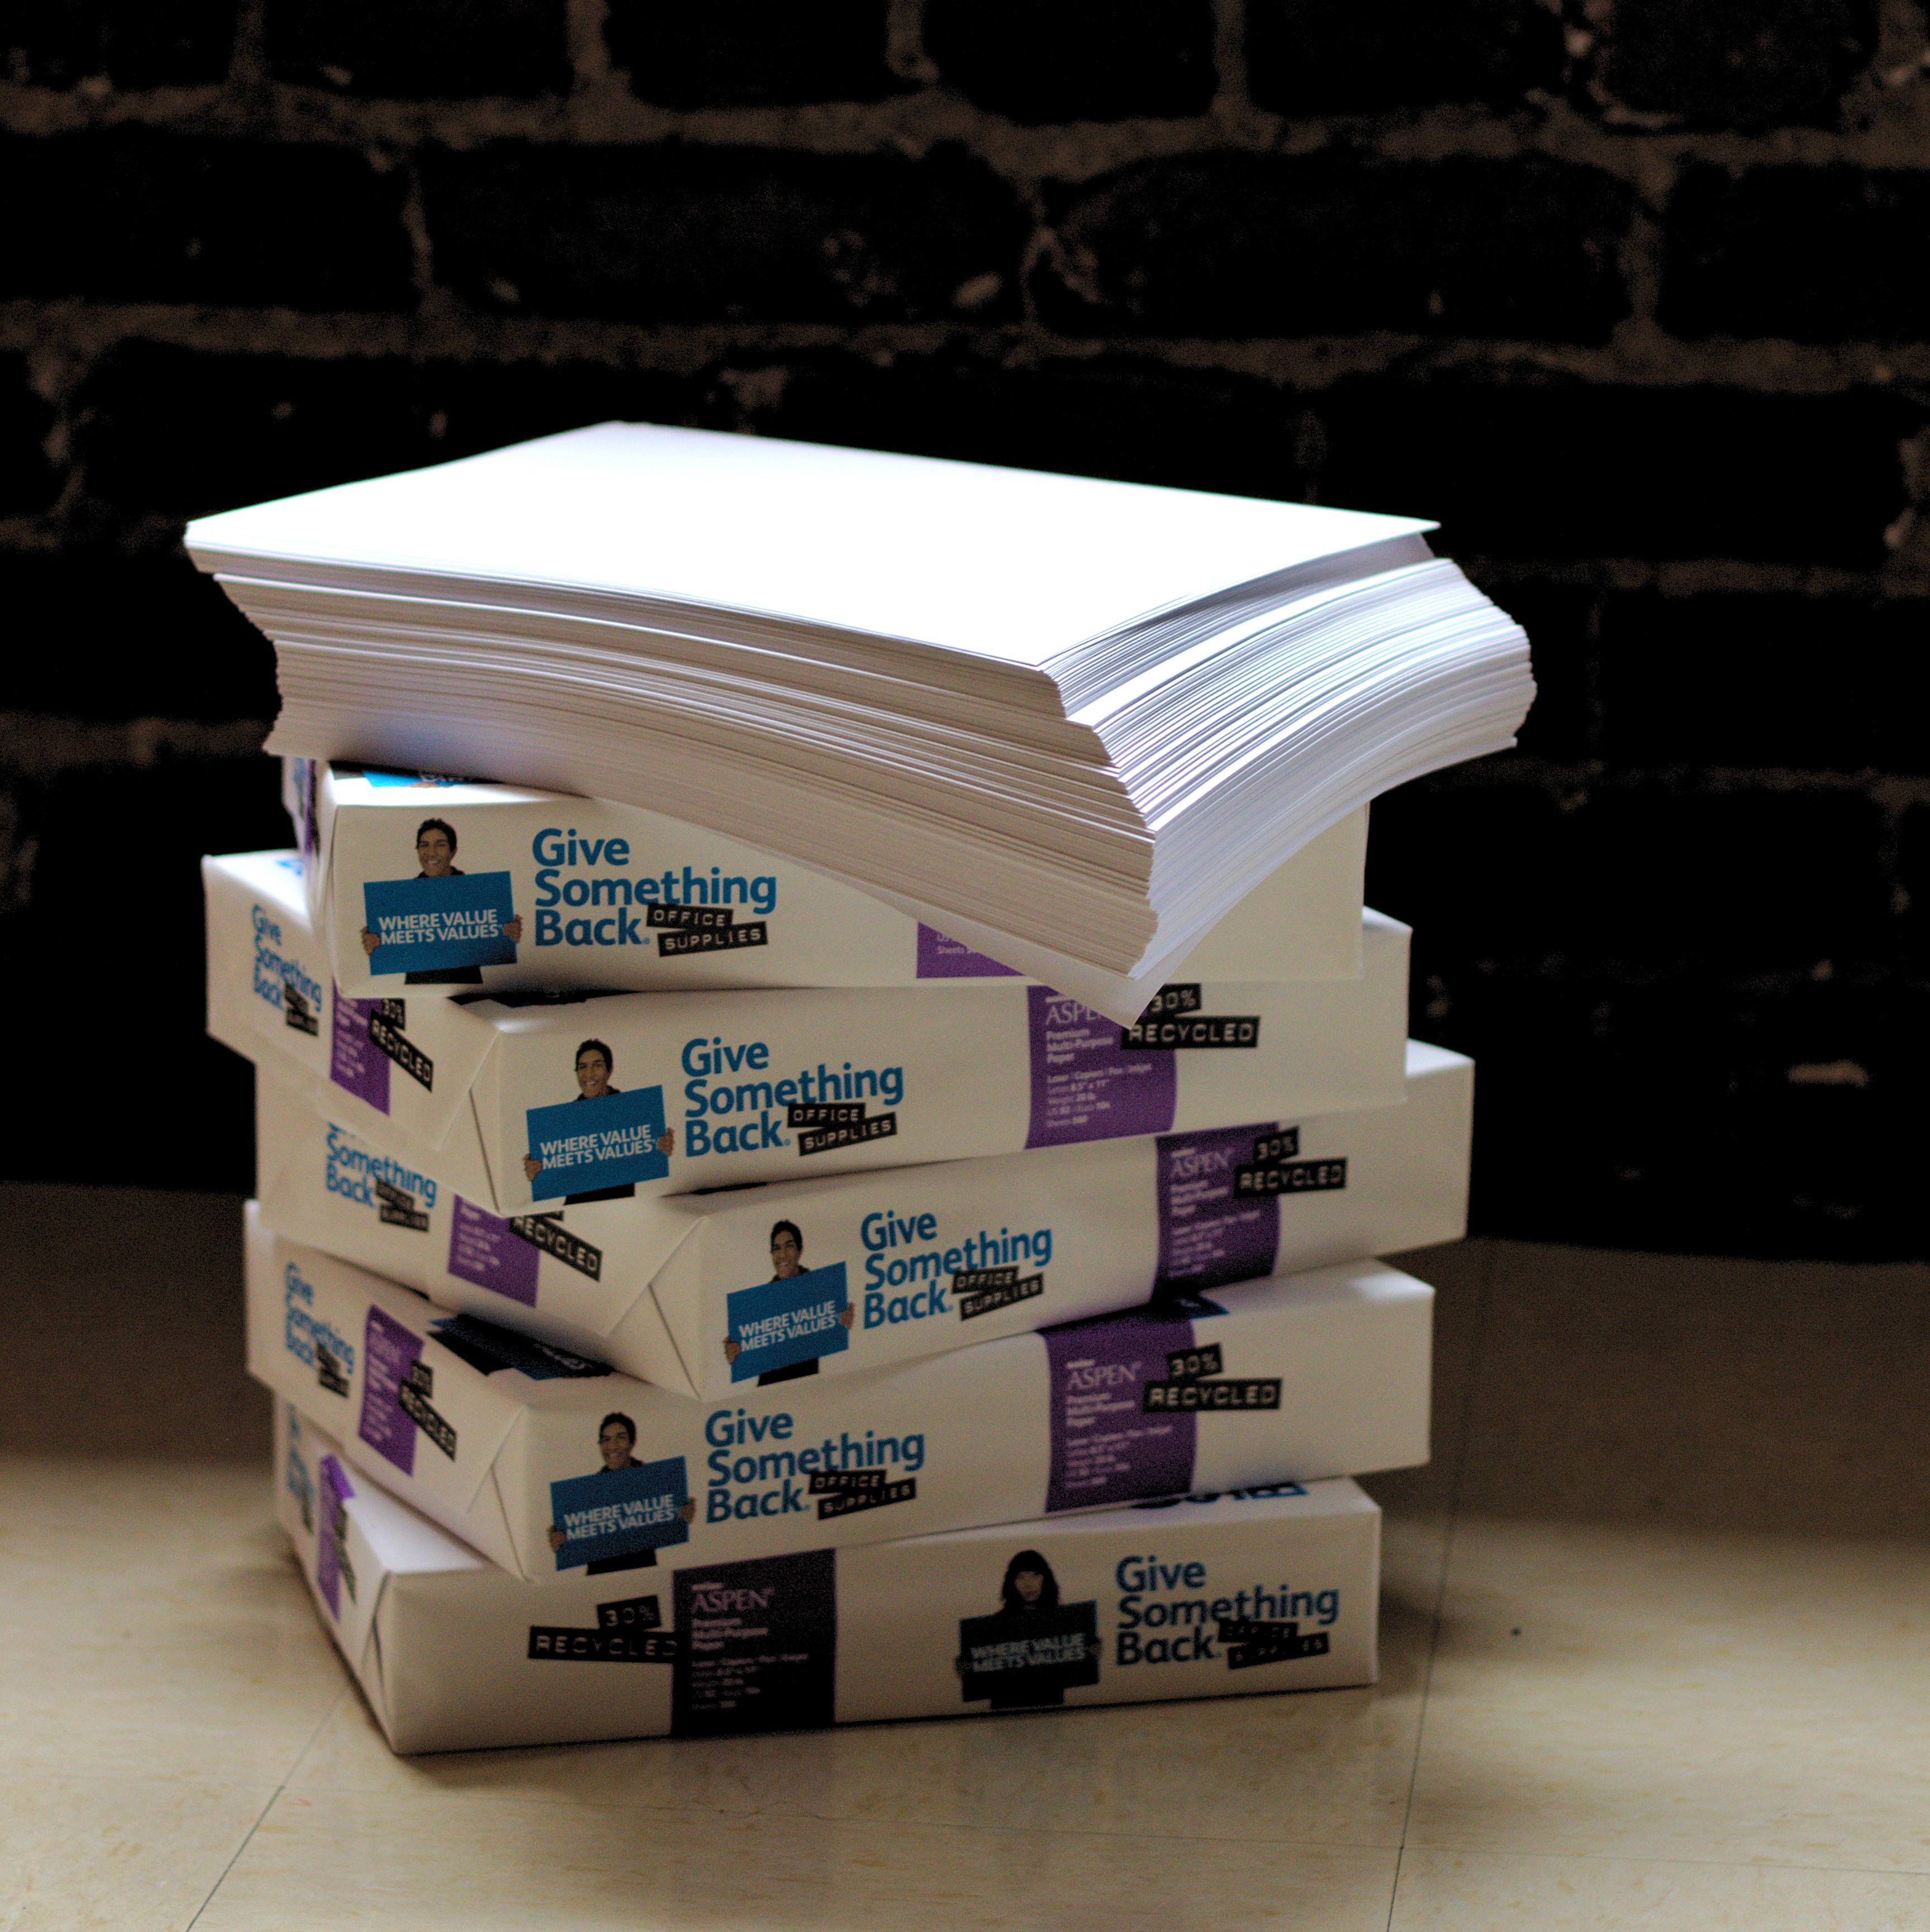
\includegraphics[width=0.3\textwidth]{./chapter18/figure14}\end{center}
  \begin{inparaenum}[(a)]
\item adding reactants %\ce{->}
\item increasing temperature %\ce{<-}
\item decreasing temperature% \ce{->}
 \end{inparaenum}
\end{question}
\begin{solution}
  \begin{inparaenum}[(a)]
\item  \ce{->}
\item  \ce{<-}
\item  \ce{->}
 \end{inparaenum}
\hspace{0.1cm}\end{solution}\stepcounter{numA}%%%%%%%%%%%%



%%%%%PROBLEM
\begin{question}[ID=\the\value{numA}]\SetQuestionProperties{section-title=\nameref{sec:units}}
According to Le Ch\^{a}telier principle indicate whether the following reaction will shift in the direction of products (\ce{->}) or reactants (\ce{<-}) after the following changes: 
  \begin{center}\includegraphics[width=0.3\textwidth]{./chapter18/figure15}\end{center}
  \begin{inparaenum}[(a)]
\item   adding products %\ce{<-}
\item removing products%\ce{->}
\item increasing temperature %\ce{->} 
 \end{inparaenum}
\end{question}
\begin{solution}
  \begin{inparaenum}[(a)]

\item    \ce{<-}
\item  \ce{->}
\item  \ce{->} 
 \end{inparaenum}
\hspace{0.1cm}\end{solution}\stepcounter{numA}%%%%%%%%%%%%









\end{multicols*}

\newpage
\begin{answersenvironment}
\begin{minipage}[c]{1\textwidth}
\begin{localsize}{10}
{\Large \bf Answers}
\SetupExSheets{
  headings = inline-nr , % numbered and inline
  counter-format = qu) , % numbers 1) 2) ... 
}
%\printsolutions 
 %\printsolutions[byID={1,3,5,7,9,11,13,15,17,19,21,23,25,27,29,31,33,35,37}]
\end{localsize}
\end{minipage}\end{answersenvironment}
\end{document}

